\section{$L_1$因子分析}

\subsection{因子分析简介}
因子分析是主成分分析的推广和发展,它也是多元统计中广泛使用的一种降维方法。
因子分析研究相关矩阵或者协方差矩阵的内部依赖关系,它将多个变量综合为少数几个因子,
以再现原始变量和因子之间的关系。

因子分析最早由英国心理学家Charles Spearman提出,最早用于智力测验得分数据的分析中。
现在因子分析在心理学、社会学、经济学等学科都取得了广泛应用。
\subsubsection{正交因子模型}

设$\bm{X} = (X_1, X_2, ..., X_p)^T$是可观测的随机向量,$\mathbb{E}\bm{X} = \bm{\mu}$,
$\mathbb{D}(\bm{X}) = \bm{\Sigma}$,设$\bm{f} = (f_1, f_2, ..., f_m)^T\\ (m <p)$为不可观测的随机向量,且
$\mathbb{E}\bm{f} = 0$,$\mathbb{D}(\bm{f}) = \bm{I}_m$(即$\bm{f}$的各分量方差为1,且互不相关)。最后,设
$\bm{e} = (e_1, e_2, ..., e_p)^T$和$\bm{f}$互不相关,并且
$$
    \mathbb{E}(\bm{e}) = \bm{0}\mbox{,}\mathbb{D}(\bm{e}) = diag({\sigma _1}^2, ..., {\sigma _p}^2)
    \mbox{为对角矩阵。}
$$
假设随机向量$\bm{X}$满足以下模型:
\begin{equation*}
\left\{
\begin{array}{clr}
    X_1 - \mu_1 = a_{11}f_1 + a_{12}f_2 + ... + a_{1m}f_m + e_1, \\
    X_2 - \mu_2 = a_{21}f_1 + a_{22}f_2 + ... + a_{2m}f_m + e_2, \\
    ... \\
    X_p - \mu_p = a_{p1}f_1 + a_{p2}f_2 + ... + a_{pm}f_m + e_p,
\end{array}
\right.
\end{equation*}
我们称该模型为正交因子模型,矩阵表示为:
$$
    \bm{X} = \bm{\mu} + \bm{A}\bm{f} + \bm{e}
    \eqno{(2-1)}
$$
其中$f_1, f_2, ..., f_m$称为$\bm{X}$的公共因子;$e_1, e_2, ..., e_p$称为$\bm{X}$
的特殊因子。公共因子一般对$\bm{X}$的每一个分量都起作用,而$e_i$一般仅仅对$X_i$起作用。
并且各个特殊因子之间以及特殊因子和所有公共因子之间都是不相关的。
其中$\bm{A} = (a_{ij})_{p \times m}$是待估计的系数矩阵,称为因子载荷矩阵。
$a_{ij}$称为第$i$个变量在第$j$个因子上的载荷,它反映了第$i$个变量在第$j$个因子上的相对重要性。

% 设$p$维随机向量$X=(X_1, X_2, ..., X_p)^T$的数学期望为$\mu = (\mu_1, \mu_2, ..., \mu_p)^T$,
% 协方差矩阵为$\Sigma$,假设$X$线性依赖于少数几个不可观测的随机变量$f_1, f_2, ..., f_m(m < p)$,和$p$个随机
% 误差项$e_1, e_2, ..., e_p$,一般称$f_1, f_2, ..., f_m$为公共因子,称$e_1, e_2, ..., e_p$为特殊因子或
% 误差,因子模型有如下表达式:
% $$ X = \mu + Af + e \label{a}  \eqno{(2-1)}$$
% 其中$f = (f_1, f_2, ..., f_p)^T$为因子,$A$是因子载荷矩阵,$e = (e_1, e_2, ..., e_p)^T$是特殊因子。
% 在式($2-1$)中,随机向量$X$围绕均值的波动由公共因子的线性组合加上一个特殊因子解释。
% 经典因子模型假设相互独立,$e_1, e_2, ..., e_p$相互独立并且$f$和$e$的样本之间相互独立。

\subsubsection{动态因子模型}

经典因子模型即正交因子模型提出后,迅速成为在心理学、社会学等多个学科内得到了广泛的使用。
然而因子模型在计量经济学研究领域的应用出现较晚,这可能是因为经典因子模型主要用于处理截面数据,
而计量经济学,尤其是宏观计量经济学的主要研究对象为时间序列数据。

Geweke与Sargent等人首先在计量经济学领域提出了动态因子模型,
动态因子模型是经典因子模型在时间序数据上的延伸,它提供了从维数众多的经济时间序列数据中提取公共因子来研究和解释
经济波动的手段。
动态因子模型的基本思想是:宏观经济具有周期性的波动是通过一系列经济变量的活动来传递和扩散的,
任何一个经济变量本身的波动都不足以代表宏观经济的整体波动。对于经济波动的研究需要从多个具有相依性的经济变量同时着手。
因此,需要从一国许多经济时间序列数据中估计出驱动各变量波动的共同动态因子,并且给出解释。
动态因子模型已经成为判别和分析经济周期波动的有效工具。

令$\bm{X}_t = (\bm{X}_{1t},\bm{X}_{2t}, ..., \bm{X}_{pt})^T$为一组宏观经济变量在$t$时刻的水平,并且$\bm{X}_t$可以表达为如下形式:
$$ \bm{X}_t = \lambda(L)\bm{f_t} + e_t \eqno{(2-2)}$$
其中,$\bm{f}_t$ 为$q\time 1$ 维的动态因子向量,$\lambda(L)$为由$s$阶滞后多项式算子组成的$p \times q$矩阵。
动态因子模型通常假设动态因子向量服从某一个向量随机过程。即动态因子模型
不仅允许观测变量受因子滞后项的影响,而且也允许因子本身具有独立的动态演化过程。

\subsubsection{近似因子模型}
在近似因子模型出现以前,DFM 主要应用于仅 包含几个总体宏观经济变量的小型数据集。这主要 是由于经济学家们假定影响所有变量的普遍性结构
冲击是经济变量协同变动的原因。然而在包含成百 上千个变量的大型经济数据集中,往往存在仅影响 某一组变量的部门冲击或局部冲击,
若根据经济理 论将这些非普遍性冲击归于异质性部分,则会造成 异质性部分截面相关,这又违背了经典因子模型中 异质性部分相互正交的假定。

因此,Chamberlain 和 Rothschild放弃 异质性部分的协方差矩阵为对角阵 的假定,允许异质性部分存在一定程度的截面相关, 
模型假设允许$f_t$的各个分量$f_1, f_2, ..., f_m$具有相依性,$e_1, e_2, ..., e_p$可以不独立,
并且允许$f_t$,$e_t$具有时间序列相依性。从而将模型扩展为了为动态近似因子模型。

% 通过放宽模型假设和形式变换,可以将动态因子模型转变为在经济变量预测中更加实用的静态近似因子模型。
% 令$X_t = (X_{1t},X_{2t}, ..., X_{pt})^T$为一组宏观经济变量在$t$时刻的水平,并且$X_t$可以表达为如下形式:
% 其中$f_t$是$q$维的动态相依因子向量,$\lambda(L)$为由$s$阶滞后多项式算子组成的$p \times q$矩阵。近似因子
% 模型的模型假设允许$f_t$的各个分量$f_1, f_2, ..., f_m$具有相依性,$e_1, e_2, ..., e_p$可以不独立,


% 令某一个经济指标$y$在$t+h$时刻的水平为$y_{t+h}$,则其预测值由式($2-4$)给出:
%     $$X_t = AF_t + e_t $$
%     $$y_{t+h} = \beta F_t + \beta _yy_t + \varepsilon _{t+h} \eqno{(2-4)}$$
% 其中$\beta F_t$包括了近似因子$t$时刻的当期项和滞后项,$\beta _yy_t$代表了指标$y$受自身滞后项的影响,$\varepsilon _{t+h}$
% 为预测误差。

\subsection{因子模型的估计}
% 在$2.1$节中提出,使用因子模型进行分析的关键是找出最具贡献的因子,而关键步骤就是要估计因子载荷矩阵。
% 对于($2-1$)中的因子模型,假设我们已知$p$个相关变量的观测值
% $$\bm{X}_{(i)} = (x_{i1}, ..., x{i_p})^T (i = 1, 2, ..., n)$$
\subsubsection{正交因子模型的估计}
对于正交因子模型,
在因子载荷矩阵$\bm{A}$中,我们计算各列的平方和,记为$q_j^2$,即
$$
    q_j^2 = \sum_{i=1}^p a_{ij}^2 (j = 1, 2, ..., m)
$$
$q_j^2$表示第$j$个公共因子$f_j$对$\bm{X}$的所有分量的总影响,称为公共因子$f_j$对$\bm{X}$的
方差贡献。因此如果我们列出$\bm{A}$的所有列平方和,按照方差贡献大小就可以选出最有影响的公共因子。
因此因子分析的关键步骤就是估计出因子载荷矩阵。

对于正交因子模型可以通过主成分法、主因子法和极大似然法来估计因子载荷矩阵。不可观测的公共因子有时候也需要进行估计,
例如用来诊断因子模型或者作为进一步分析的原始数据,这就需要我们给出因子得分,一般在得出了因子载荷矩阵之后,
对于因子得分,可以通过加权最小二乘法(巴特莱因子得分)或者通过回归法(汤普森因子得分)进行估计。

\subsubsection{动态因子模型的估计}
动态因子模型的提出者Geweke和Sargent等人都是使用频域方法估计模型,这种方法不能够直接估计出动态因子$\bm{f}_t$,
因此也就不能将因子作为预测或者扩展模型等用途。使得动态因子模型的应用收到限制。
由于动态近似因子模型估计困难,因此在预测中,往往使用模型的静态形式:
$$X_t = AF_t + e_t \eqno{(2-3)}$$
式($2-3$)中,$F_t$是$m$维向量,称为静态因子,即$F_t$仅在当期影响$X_t$(因为$F_t$包括了动态因子$f_t$的当期项和
滞后项),它本身可以不具有经济学含义。$A$是因子载荷矩阵。本文采用式($2-3$)中的模型进行宏观经济指标的预测。

对于静态形式的估计,Stock和Watson于1989年最早提出了一种方法:这种方法采用
Kalman 滤波构造似然 函数,并采用极大似然方法来估计参数。
这种方法的 优点是: 在误差项服从正态分布的假定下,能够得到 因子的有效估计量。
然而,由于在估计参数过程中 会应用到非线性数值优化算法,而待估参数的个数与变量维数$p$成比例,
限于当时的计算能力,这种方法只能用于处理低维的精确动态因子模型。

针对维数很高的宏观经济变量,Stock和Watson于2002年给出了一种非参数的方法,并且得到广泛使用。
这种方法使用主成分分析法进行估计,对式($2-3$),因子载荷矩阵$\bm{A}$的估计量$\hat{\bm{A}}$即为
$\bm{X}_t$的样本协方差矩阵$$\hat{\bm{\Sigma}}_{\bm{X}} = \frac1{n}\sum_{t=1}^n\bm{X_t}\bm{X_t}^T$$的前
$r$个最大特征值所对应的特征向量组成的$p\times r$维矩阵,因子的主成分估计量为:
$$ \hat{\bm{F}}_t = \frac1{n}\hat{\bm{A}}\bm{X}_t $$

主成分估计量具有一系列良好的性质。例如, 在$p \rightarrow \infty$, $n \rightarrow \infty$ 且 $p^2 / n \rightarrow \infty$
的条件下,主成分估计量$\hat{\bm{F}}_t$是因子空间的一致估计量,且在随后的建模 过程中可以当作观测到的数据。
\subsubsection{主成分分析法}

\subsubsection{奇异值分解} 
述因子模型中,需要估计因子载荷矩阵$A$和因子得分矩阵$F^T$。容易发现,这个问题等价于以下矩阵分解问题:
$$ X_{p\times n} = \hat{A}_{p\times m} \hat{F^T}_{m\times n} \eqno{(2-5)}$$
$$
\hat{A}_{p\times m}, \hat{F^T}_{m\times n} = \underset{A,F^T}{\operatorname{arg\ min} } \|X - AF^T\|_{L_2}
 = \underset{A, F^T}{\operatorname{arg\ min}} \sum_{i=1}^p \sum_{j=1}^m (x_{ij} - a_i^Tf_i)^2 \eqno{(2-6)}$$

\subsection{$L_1$因子分析}
使用最小二乘具有计算简便的特点,
尽管在求解某些问题时用最小二乘估计求解可以得到比较令人满意
的效果, 但最小二乘法也存在一些局限性, 比如, 当收集的数据较少或者具有较多的缺失数据
并且数据中夹杂有异常点时, 用最小二乘法所得的结果就令人难以接受, 在此情况下应用所得到到的回归方程或模型进行预测或者拟合时, 
则预测或拟合的精度是相当低的, 甚至根本不能使用。
正因为最小二乘法对数据中的异常值十分敏感,当数据中具有较多离群值时,通过最小二乘、PCA和SVD方法,得到的估计结果也会受到较大影响。
这里我们提出基于$L_1$范数的方法,来增加估计的健壮性。


\subsubsection{$L_1$范数及其稳健性}
设$\bm{X} = (X_1, X_2, ..., X_p)^T$为一$p$维随机变量,$Y$为响应变量,$\bm{\beta}$为回归系数。
假设我们观察到$i.i.d. $样本$(\bm{X}_1, \bm{X}_2, ..., \bm{X_n})$和$(Y_1, ..., Y_n)$,我们一般使用$\bm{\beta}$
的最小二乘估计量
$$\hat{\bm{\beta}} = \underset{\bm{\beta}}{\operatorname{arg\ min}} \sum_{i=1}^n\|Y_i - \bm{X}^T_i\bm{\beta}\|_{L_2}
=\underset{\bm{\beta}}{\operatorname{arg\ min}} \sum_{i=1}^n(Y_i - \bm{X}^T_i\bm{\beta})^2$$

在稳健统计中,我们经常使用其他的目标函数,例如使用$L_1$范数来代替$L_2$,
$$\hat{\bm{\beta}} = \underset{\bm{\beta}}{\operatorname{arg\ min}} \sum_{i=1}^n\|Y_i - \bm{X}^T_i\bm{\beta}\|_{L_1}
=\underset{\bm{\beta}}{\operatorname{arg\ min}} \sum_{i=1}^n|Y_i - \bm{X}^T_i\bm{\beta}|$$

如图所示,通常使用$L_1$范数在线性回归中可以有效避免离群值造成的干扰。
\begin{figure}[H]
    \centering
    \begin{minipage}[t]{0.48\textwidth}
    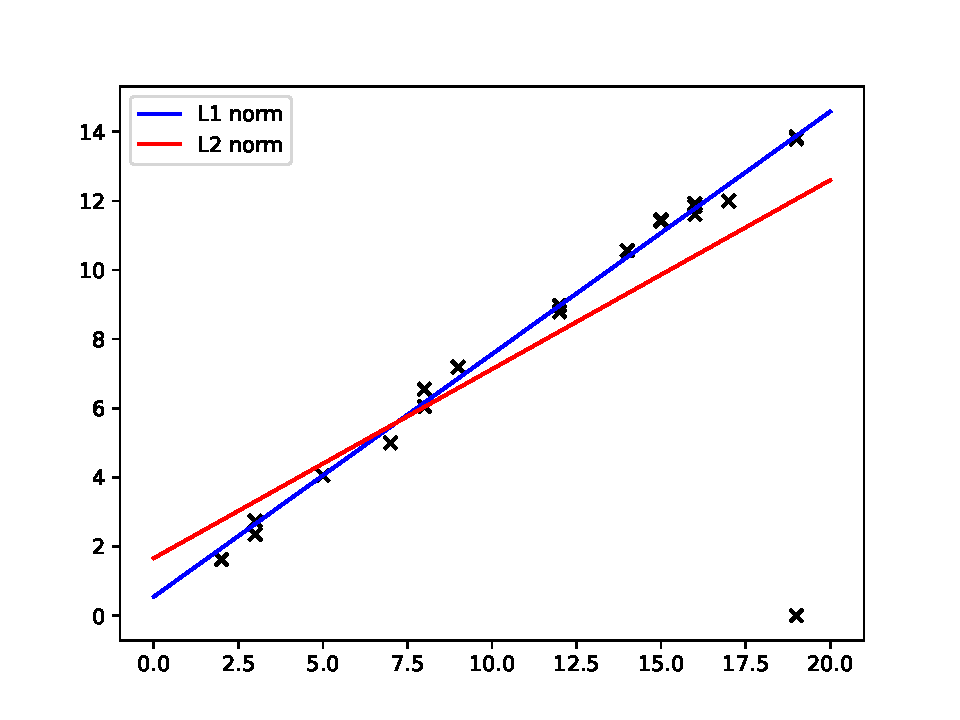
\includegraphics[width=8cm]{pics/l1-l2-diff2.pdf}
    \end{minipage}
    \begin{minipage}[t]{0.48\textwidth}
    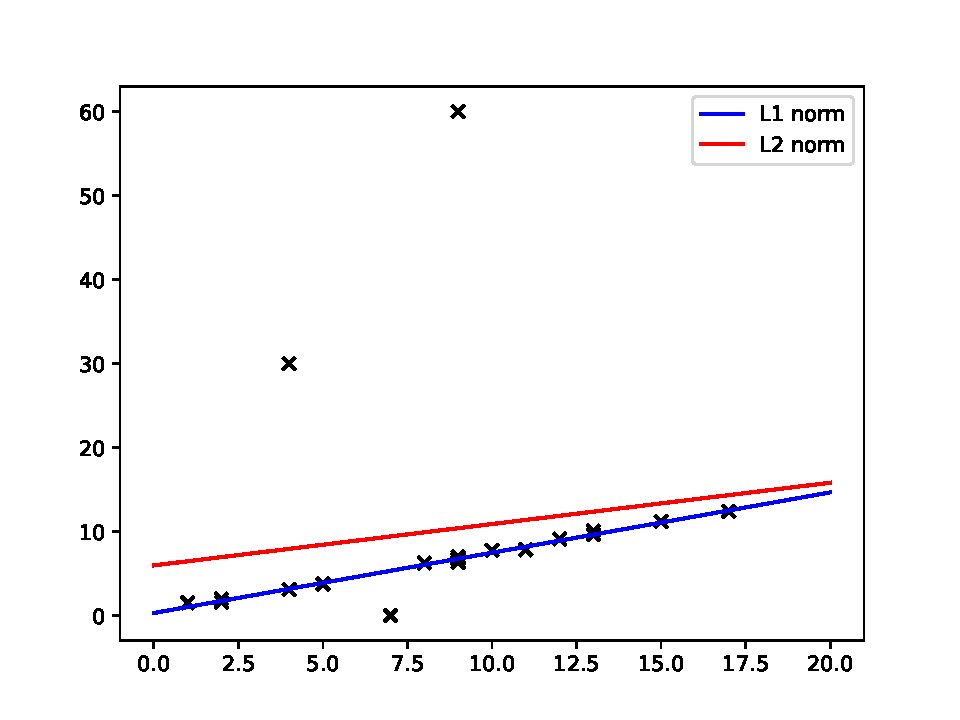
\includegraphics[width=8cm]{pics/l1-l2-diff.pdf}
    \end{minipage}
    \caption{\small 如图所示,在简单的线性模型的拟合中,出现一个离群值就可以导致最小二乘法拟合出现明显的偏差;
    而含有较多离群值时最小二乘法拟合变得很不可靠;而采用$L_1$范数则具有相当稳健性。}
    \label{fig2.1}
\end{figure}

\subsubsection{$L_1$因子分析算法}
将式($2-6$)中的目标函数更换为使用$L_1$范数,可得
$$\hat{A}_{p\times m}, \hat{F^T}_{m\times n} = \underset{A,F^T}{\operatorname{arg\ min} } \|X - AF^T\|_{L_1}
= \underset{A, F^T}{\operatorname{arg\ min}} \sum_{i=1}^p \sum_{j=1}^m |x_{ij} - a_i^Tf_i| \eqno{(2-7)}$$
其中$\|.\|_{L_1}$表示矩阵的$L_1$范数。

式($2-7$)中定义的问题不是一个凸优化问题。但是一旦矩阵$A$或者$F^T$固定为常数,那么该问题就成为了一个凸优化问题,
可以找到全局最优解。这启发我们可以使用交替优化的方法求解这个优化问题,即每一步固定$A$或者$F^T$的值,来求解另一个
参数。

$$
F^{(t)} = \underset{F}{\operatorname{arg\ min}} \|X - A^{(t-1)}F^T \|_{L_1} \eqno{(2-8a)}
$$
$$
A^{(t)} = \underset{A}{\operatorname{arg\ min}} \|X - AF^{T(t)}\|_{L_1} \eqno{(2-8b)}
$$

我们改写式($2-8a$)中的目标函数,
$$
E(F) = \|X - A^{(t-1)}F^T \|_{L_1} = \sum_{j=1}^{n}|x_j - A^{(t-1)}f_j| \eqno{(2-9)}
$$
其中$x_j$是矩阵$X$的第j列,$f_j$是$F^T$的第j列。于是式($2-8a$)中的问题可以分解为$n$个独立的子优化问题,
求解相应的$f_j$:
$$
    f_j = \underset{\theta}{\operatorname{arg\ min}} |A^{(t-1)}\theta - x_j|
    \eqno{(2-10)}
$$
式($2-10$)的全局最优解可以通过求解下面的线性规划问题得到:
$$
    \underset{\theta, t}{\operatorname{min}} 1^T t
$$
$$
    s.t. -t \leq A^{(t-1)}\theta - x_j \leq t \eqno{(2-11)}
$$
线性规划问题的计算性能取决于未知变量的个数和和约束的个数。这里的$n$个子优化问题共享了$A^{(t-1)}$,
减少了一定的计算量。但是每一个子优化问题都要面临$p$个约束条件和一个
$p$维未知变量,当$x_j$是一个维数非常大的向量时$p$很大),每一个子问题的求解仍然需要大量计算。虽然现在已经
发展出了有效的处理多变量多约束线性规划问题的方法,但是在因子分析的场合下我们仍给出一个性能更好的方法来代替
这里的线性规划。这个方法将在第三章中讨论。

\subsubsection{缺失值处理}
在使用PCA和SVD时我们需要对矩阵$X$进行缺失值插补,然后才能进行计算。
在$L_1$算法中我们不需要进行缺失值插补,在式($2-11$)中,遇到$x_j$具有缺失值的场合,我们直接舍弃相应的
约束条件即可。
我们改写式($2-9$),
$$E(F) = \sum_{i=1}^d \sum_{j=1}^n |x_{ij} - a_i^Tf_j|$$
如果某个项$x_{ij}$缺失,我们直接舍弃目标函数中的对应累加项,在上述算法中对应的做法就是直接删除($2-11$)中的一个约束条件。

\subsubsection{$L_1$因子分析算法}
我们已经发现可以通过交替优化的方法求解式($2-7$)中的优化问题,下面我们更加详细地讨论$L_1$因子分析算法一些细节和具体实现步骤。

(一)初始化

和其他所有的迭代算法一样,在算法开始时,首先我们需要给$A$一个初始值$A^{(0)}$。对于$A$可以采用简单随机数进行初始化,这里我们
为了加快收敛速度,可以使用经过缺失值插补(这里我们使用均值插补)后通过PCA算法进行得到的因子载荷矩阵作为$A^{(0)}$。
在本章后续小结的实验中我们可以发现,在含有大量缺失值和离群值的条件下,两种不同的初始化方法最终结果差异并不大。

(二)收敛性

因为目标函数$E(A, F) = \|X - AF^T\|_{L_1}$在每一个交替的优化步骤中都递减,并且$E(A,F)$具有下界($\geq 0$)。
因此交替优化算法一定收敛。因此我们可以设定一个收敛域值来停止迭代,这里我们设置终止条件:
    $$ \theta(a_i^{(t)}, a_i^{(t-1)}) <  \alpha $$
这里$\theta(a, b)$表示向量$a$和$b$的夹角;其中$a_i$是$A$或者$F$的第i列;$\alpha$是一个很小的正数。

(三)算法步骤

下面我们给出$L_1$因子分析算法的计算步骤:

1.初始化:给出$A$,$\Sigma$的初始值$A^{(0)}$,$\Sigma^{(0)} = I$,(其中$\Sigma$为一对角矩阵,
$I$为单位矩阵);

2.交替凸优化:对于迭代次数$t = 1, ..., $收敛:
$$F^{(t)} = \underset{F}{\operatorname{arg\ min}} \|X - A^{(t-1)}\Sigma^{(t-1)}F^{T}\|_{L_1}$$
$$A^{(t)} = \underset{A}{\operatorname{arg\ min}} \|X - A\Sigma^{(t-1)}F^{T(t)} \|_{L_1}$$
\begin{equation*}
    \text{归一化:}\left\{
                 \begin{array}{clr}
                 N_a = diag(A^{(t)T}A^{(t)})\\
                 N_f = diag(F^{(t)T}F^{(t)})\\
                 F^{(t)} \leftarrow F^{(t)}N_f^{-1}\\
                 A^{(t)}\leftarrow A^{(t)}N_a^{-1}\\
                 \Sigma^{(t)} \leftarrow N_a\Sigma^{(t-1)}N_f\\
                 \end{array}
    \right.
\end{equation*}

3.输出结果:$F \leftarrow F\Sigma^{1/2}$,$A \leftarrow A\Sigma^{1/2}$

\subsection{稳健性实验}
为了检验$L_1$因子分析算法在处理含有大量离群值和缺失值的数据时的稳健性,我们进行模拟实验,来对比采用$L_1$因子分析算法
和PCA因子分析,SVD因子分析以及采用$L_2$目标函数这几种方法的效果。

\subsubsection{数据准备}
为了进行模拟实验,我们首先需要随机产生一个高维低秩的矩阵来模拟高维宏观经济数据集。
我们产生一个$n$维方阵$M$,其中每一个随机元素均服从$[-100, 100]$的均分分布。然后我们对方阵$M$进行奇异值分解
,$M = U\Sigma V^{T}$。假设我们需要产生的低秩矩阵的秩为$r$,则$$X = U_{(:,1:r)}\Sigma_{(1:r,1:r)}V^T_{(:,1:r)}$$
即为我们得到的模拟高维低秩矩阵。

之后我们可以设置一定比例的缺失值和离群值,首先我们在矩阵的左下角剔除部分元素。在剩下的元素中,我们随机选取一部分
然后重新产生随机元素,每个元素服从$[-2000,2000]$上的均匀分布。图2.1展示了一个$30\times30$秩为3的
矩阵在模拟了缺失值和离群值后的情况。

\begin{figure}[H]
    \centering
    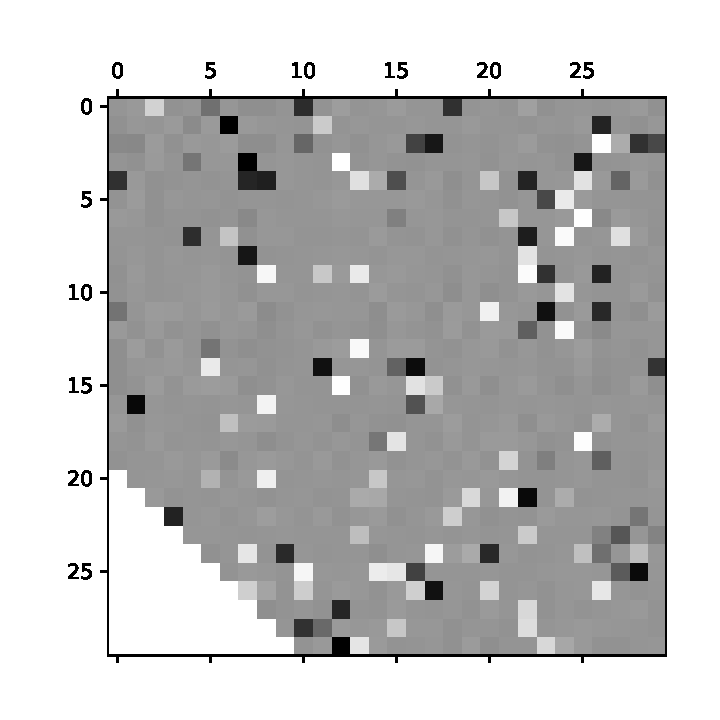
\includegraphics[width=.5\textwidth]{pics/matrix.pdf}
    \caption{\small $30\times30$的模拟矩阵,左下角白色代表缺失值,图中灰度越深代表元素的绝对值越大,因此深黑色的点代表了离群值}
    \label{fig2.1}
\end{figure}